\section{System Description}

The device studied throughout this project is a linear system with a static nonlinear feedback loop. It has a single input and a single output and the feedback is known to follow the input-output relation given by
\begin{equation}
    y(t) = u^3(t).
    \label{eq:NL_feedback}
\end{equation}

The objective will be to identify the linear part of the system and to have a measure of the nonlinearity and noise levels. The knowledge of~(\ref{eq:NL_feedback}) will not be used, except for a small parenthesis about odd and even nonlinearities.

The measurement device (referred to as the \textit{PXI setup}) allows to send only multisines and their RMS value cannot exceed $1$~V. Its ADCs have a range that can be chosen and can sample at high frequencies ($> 1$~GHz).

This report deliberately focusses on the theoretical points and the results rather than the implementation because the Matlab scripts and the measured data are available on GitHub\footnote{https://github.com/e-colot/LTI-identification}. 





\section{Excitation Signal}

Before making any useful measurement, the parameters of the excitation signal must be chosen to match to the DUT parameters.The rms of the applied signal must indeed be determined to use the full range of the ADC while avoiding saturation of the system. The poles of the system must also be roughly known to determine the band of interest, making sure that the system's dynamics are measured.



\subsection{Band of Interest}
\label{sec:Band_of_interest}

To determine the sampling frequency, a multisine excited up to $40$~kHz has been applied to the DUT. Both input and output of the system are shown in the frequency domain in Fig.~\ref{fig:frequency_scan}.

\begin{figure}[htbp]
    \centering
    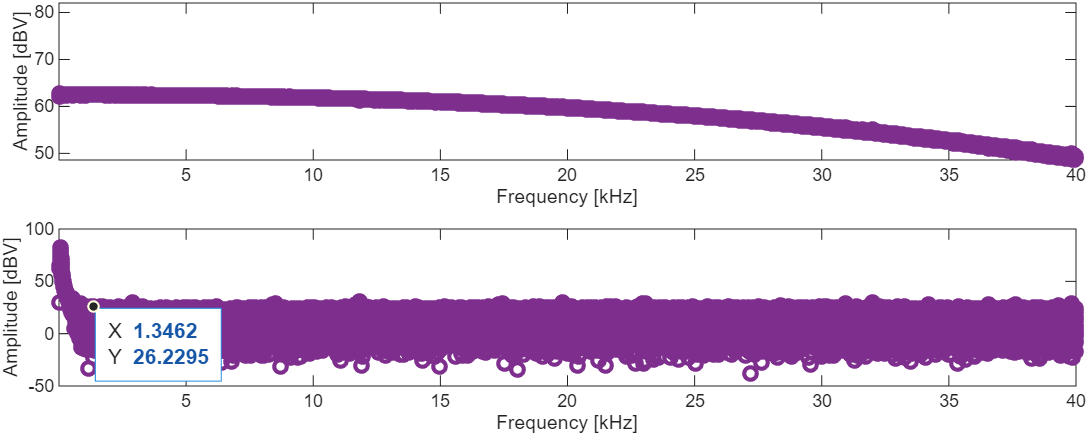
\includegraphics[width=0.48\textwidth]{Pictures/frequencyScan.png}
    \caption{Excitation spectrum (top) and output spectrum (bottom).}
    \label{fig:frequency_scan}
\end{figure}

The measured input spectrum is not flat because of the ZOH: the continuous signal is discretized by the \textit{PXI setup} and the hold operation is equivalent with a sinc filtering in frequency. This effect could be reduced with a higher sampling frequency.

The output spectrum shows that the system's dynamics happen at frequencies below $\sim 1.25$~kHz. The excitation signals used will therefore stop at this frequency. To mitigate the effect of the ZOH, the sampling frequency is set to $5$~kHz.


\subsection{Amplitude}

\begin{figure}[htbp]
    \centering
    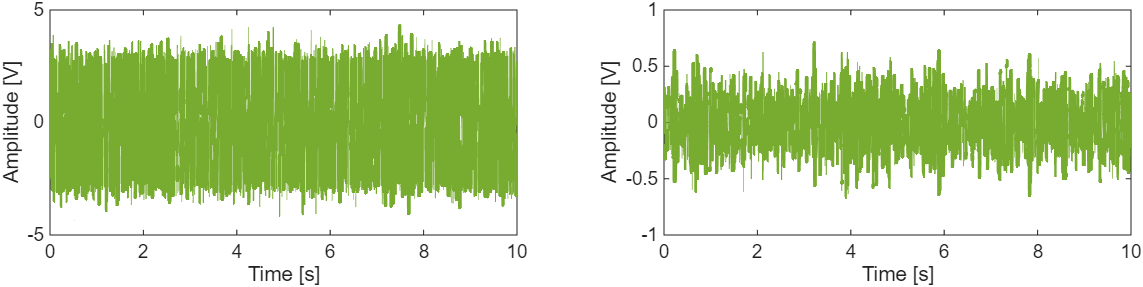
\includegraphics[width=0.48\textwidth]{Pictures/outputSignal.png}
    \caption{Excitation signal (left) and output signal (right).}
    \label{fig:output_signal}
\end{figure}

The same signal as the one measured for Sec.~\ref{sec:Band_of_interest} but is shown in the time domain in Fig.~\ref{fig:output_signal}. It can be seen that the input signal do not go higher than $5$~V and the output voltage does not cross $1$~V. This allowed to set the range of the ADCs of the \textit{PXI setup}.

\subsection{Transient Removal}

Because only multisines can be applied, every measurement is done for multiple periods and the first ones are systematically removed until the transient is removed. To check this, the difference between each period is plotted, as shown in Fig.~\ref{fig:transient_removal} and periods are removed until the shown plot is reduced to a flat curve.

\begin{figure}
    \centering
    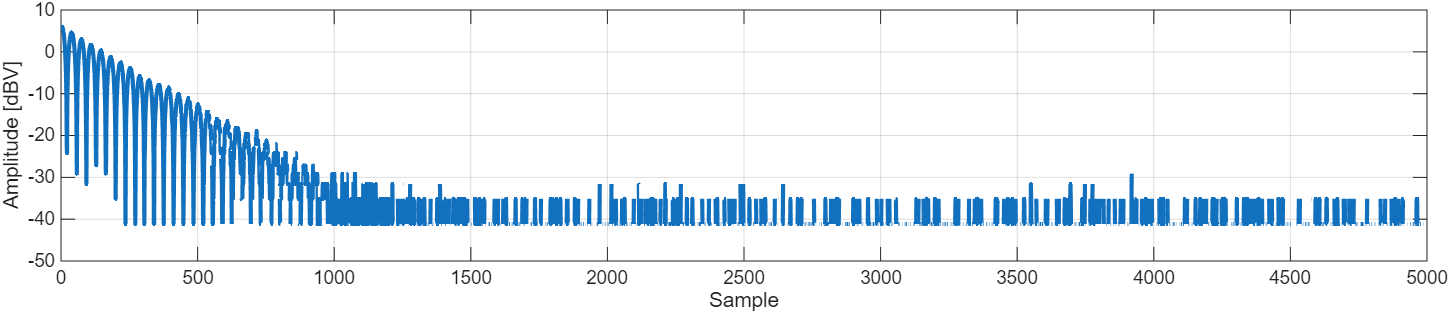
\includegraphics[width=0.48\textwidth]{Pictures/transientRemoval.png}
    \caption{Difference between $1^{\text{st}}$ and $2^{\text{nd}}$ periods of the output signal in time domain.}
    \label{fig:transient_removal}
\end{figure}








\section{Nonlinear Distortion and Noise Analysis}

Two methods are used to distinguish the nonlinear distortions from the noise. The \textit{fast method} uses a single experiment and allows to split the output spectrum in linear, nonlinear and noise contributions. The \textit{robust method} uses multiple experiments and computes an estimate of the variances of nonlinear distortion and noise together with an nonparametric estimate of the frequency response function (FRF).




\subsection{Fast Method}

The excitation signal is an odd multisine with holes. This means that only odd frequencies are excited and some of those odd frequencies are also unexcited in order to have a measure for odd nonlinear distortions. During the excitation generation, 1 odd bin out of 4 is randomly chosen to be not excited. 

The FFT of multiple periods are taken, effectively dividing the spectral resolution as $\Delta_f = f_s / N$ with a larger $N$. The added bins are not linear combinations of input frequencies and therefore only contain noise, under the assumption that the DUT is a \textit{PISPO}\footnote{period in, same period out} system.

The spectrum of the output signal is then divided into 4 categories:
\begin{itemize}
    \item \textbf{Linear}, for bins that were excited.
    \item \textbf{Even distortions}, for bins that are a combination of an even number of excited bins.
    \item \textbf{Odd distortions}, for bins that are a combination of an odd number of excited bins.
    \item \textbf{Noise}, for bins that are added by the multiple periods.
\end{itemize}

\begin{figure}
    \centering
    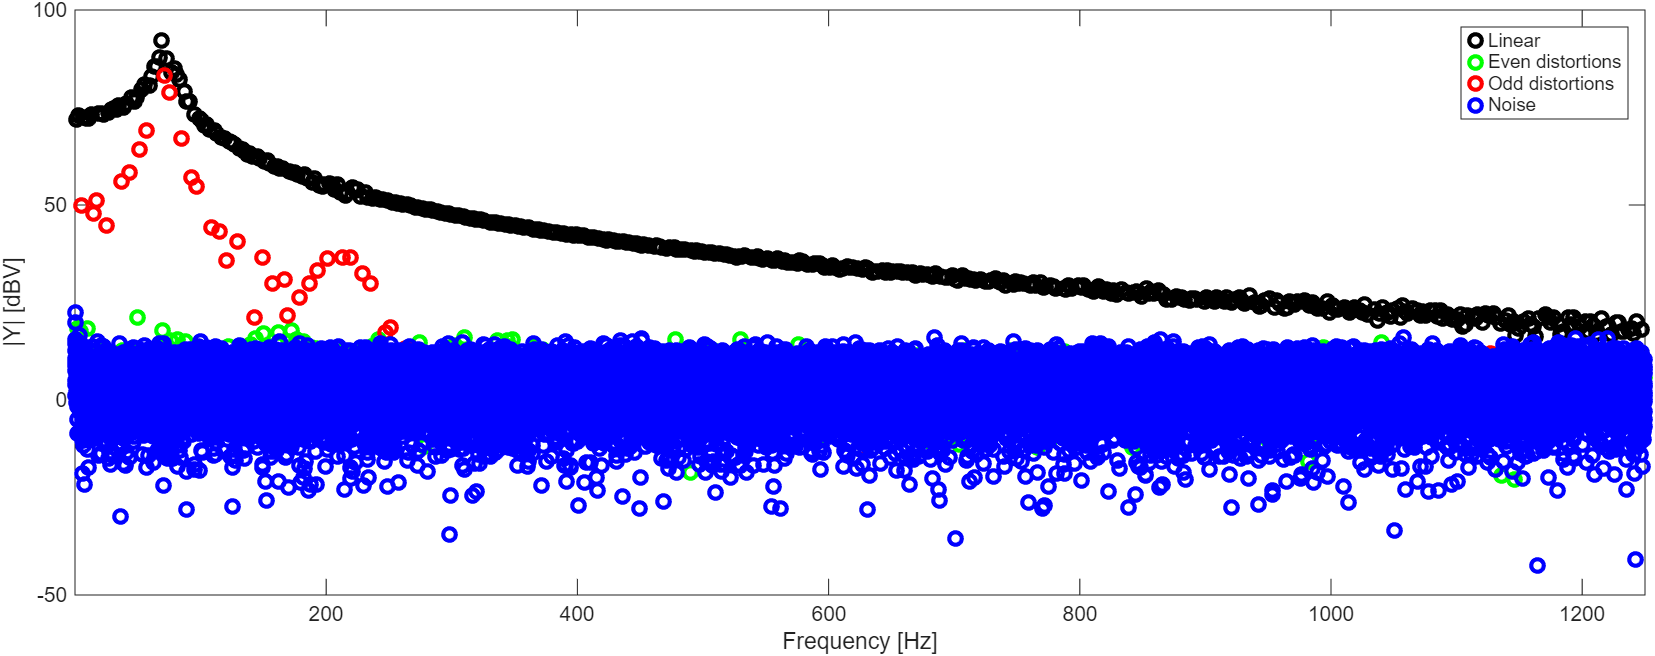
\includegraphics[width=0.48\textwidth]{Pictures/fastMethod1.png}
    \caption{Results of the fast method with the feedback given by~(\ref{eq:NL_feedback}).}
    \label{fig:fast_method}
\end{figure}

Fig.~\ref{fig:fast_method} shows that even distortion is close to the noise level and therefore does not impact much the signal. Odd distortion on the other hand is quite high and is close to the level of the linear part near its peak.

This behavior is explained by~(\ref{eq:NL_feedback}): because the third power of the output is fed back to the input, it contains sinusoids at the sum of 3 frequencies of the output. As the output only contains odd frequencies, it results in another odd frequency and the main nonlinearities therefore appears at odd bins.

To validate this explanation, the same experiment has been applied to the system with this time as feedback
\begin{equation}
    y(t) = u^2(t),
    \label{eq:NL_feedback_even}
\end{equation}

which gave the results shown in Fig.~\ref{fig:fast_method_even}.

\begin{figure}
    \centering
    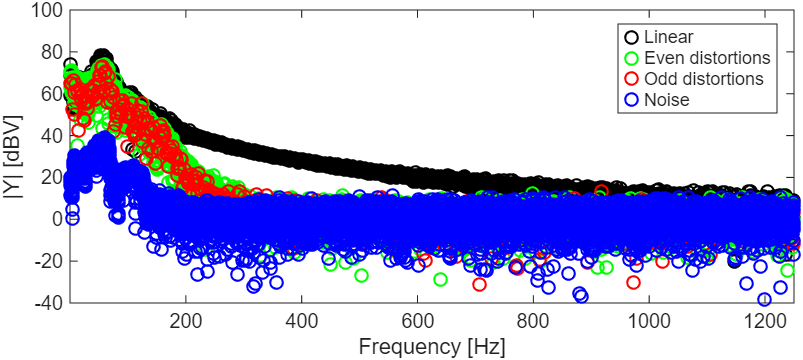
\includegraphics[width=0.48\textwidth]{Pictures/fastMethodEven.png}
    \caption{Results of the fast method with the feedback given by~(\ref{eq:NL_feedback_even}).}
    \label{fig:fast_method_even}
\end{figure}

The feedback now excites even frequencies and therefore has more even distortions than the one of Fig.~\ref{fig:fast_method}.




\subsection{Robust Method}

This method relies on computing a FRF for each of the $P$ periods and the $M$ realizations. The variance across the periods for realization $m$ is called $\hat{\sigma}^{2 [m]}_n$ and is only due to noise. This is because the nonlinear contributions are deterministic and depend only on the input signal, which is the same for the whole realization.
\begin{equation}
    \hat{G}^{[m, p]} = \frac{Y^{[m, p]}}{U^{[m]}}
\end{equation}
\begin{gather}
    \hat{G}^{[m]} = \frac{1}{P} \sum_{p=1}^P \hat{G}^{[m, p]}\\ 
    \hat{\sigma}^{2 [m]}_n = \frac{1}{P(P-1)} \sum_{p=1}^{P} \left| \hat{G}^{[m, p]} - \hat{G}^{[m]}\right|^2
\end{gather}

These noise variances on a single realization $\hat{\sigma}^{2 [m]}_n$ are then averaged across the realizations and divided by M because the averaging reduces the variance. This gives the total noise variance $\sigma^2_n$.
\begin{equation}
    \hat{\sigma}^2_n = \frac{1}{M^2} \sum_{m=1}^{M} \hat{\sigma}^{2 [m]}_n
\end{equation}

The averaged FRF of a single realization $\hat{G}^{[m]}$ does not contain noise (at least in expected value). But between realizations, they have different nonlinear effects as the phases of the excitation signals have changed. The variance between those therefore is due to nonlinear distortion and averaging it out gives a FRF estimate that is noiseless and purely linear, if $M$ and $P$ are large enough to be close to the expected value.
\begin{gather}
    \hat{G}_{\text{ML}} = \frac{1}{M}\sum_{m=1}^M\hat{G}^{[m]}\\
    \hat{\sigma}_{\text{ML}} = \frac{1}{M(M-1)}\sum_{m=1}^M\left|\hat{G}^{[m]}-\hat{G}_{\text{ML}}\right|^2
\end{gather}

A full multisine (excited up to $1.25$~kHz as explained in Sec.~\ref{sec:Band_of_interest}) has been applied to the DUT for $P=20$ periods and $M=20$ realizations. The results are shown on Fig.~\ref{fig:robust_method}.

\begin{figure}
    \centering
    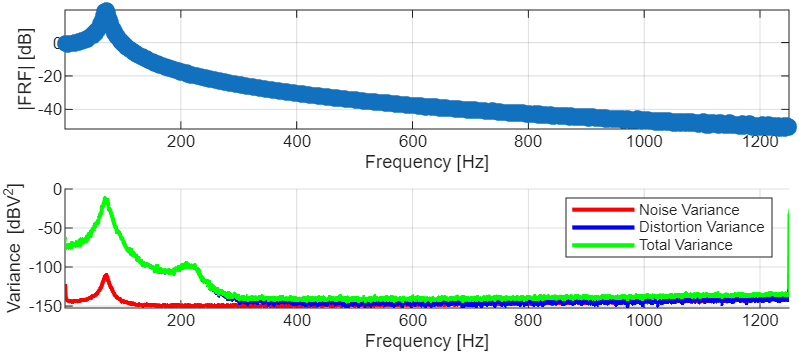
\includegraphics[width=0.48\textwidth]{Pictures/robustMethod.png}
    \caption{Results of the robust method, with the FRF estimate (top) and the estimated variances (bottom).}
    \label{fig:robust_method}
\end{figure}













\section{Best Linear Approximation}

A linearized model of the system can be determined to approximate the DUT as an LTI. The best linear approximation, or BLA, is therefore computed as the "best fit". Because nonlinear distortions are dependent on the input signal, the BLA computed here is valid for excitation signals with a similar \textit{Riemann equivalent spectrum}. 




\subsection{Nonparametric Model}
\label{sec:non_parametric_model}

The result of the robust method shown in Fig.~\ref{fig:robust_method} is, in fact, an estimated BLA and it already comes with its uncertainty. Because of the successive averaging, it should be able to remove noise and nonlinear distortions which are zero-mean\footnote{It is only true in expected value so it can only be approached using a discrete number of periods and realizations}.




\subsection{Generalities About Parametric Identification}
\label{sec:parametric_model}

Based on the nonparametric model of Sec.~\ref{sec:non_parametric_model}, a parametric model can be derived by making a choice for the model. This will be fixed by the order of the numerator and denominator of the transfer function, respectively $n_b$ and $n_a$ giving the following expression

\begin{equation}
    G(s) = \frac{\sum_{k=0}^{n_b} b_k s^k}{\sum_{k=0}^{n_a} a_k s^k}.
    \label{eq:TF_general_form}
\end{equation}

Different estimators are used but first, a few tricks are used for each of them and those are explained here.

\paragraph{Normalization by rms scaling} Each estimator has a regressor matrix ($H$ or $J$), whose columns often have different orders of magnitude. This results in a poor conditioning and gives numerical errors. To resolve this, a change of coordinates is applied with the scaling matrix $S$, which scales the columns. The original coordinates $H$ (or $J$) and $\theta$ are replaced by $\tilde{H}$ (or $\tilde{J}$) and $\tilde{\theta}$.
\begin{gather}
    y = H \times \theta \\
    \Rightarrow y = \tilde{H} \times \tilde{\theta} \qquad \text{with} \qquad \tilde{H} = H \times S
\end{gather}
\vspace{-0.8cm}
\begin{align}
    &\Leftrightarrow \tilde{\theta} = S^{-1} \times \theta\\
    &\Leftrightarrow \theta = S \times \tilde{\theta}
\end{align}
$S$ has been chosen to be a diagonal matrix with as elements the inverse of the rms of the columns of $H$, such that it is invertible
\begin{equation}
S = \operatorname{diag}\!\left( \frac{1}{\mathrm{rms}\bigl(H_{:,1}\bigr)}, \dots, \frac{1}{\mathrm{rms}\bigl(H_{:,n}\bigr)} \right).
\end{equation}

\paragraph{Use of the nonparametric estimate} All the estimators are relying on approaching the following, which arises from the definition of a transfer function. The key idea is to notice that because
\begin{equation}
    Y(k) = G_{\text{BLA}}(k) \times U(k),
\end{equation}
a clever choice of $U$ simplifies the choice of $Y$, as
\begin{equation}
    U(k) = 1 \quad \forall k \quad \Rightarrow \quad Y(k) = G_{\text{BLA}}(k).
\end{equation}

\paragraph{Forcing real valued parameters} A real system is described by real coefficients so the imaginary part of $\theta$ must be equal to $0$. The regressor must therefore be changed. $y$ and $H$ are replaced by a concatenation of their real and imaginary parts called $y_{\text{re}}$ and $H_{\text{re}}$ as follows
\begin{equation}
    y_{\text{re}} = \begin{bmatrix}
        \Re\left\{y\right\}\\
        \Im\left\{y\right\}
    \end{bmatrix}, \quad \text{and} \quad H_{\text{re}} = \begin{bmatrix}
        \Re\left\{H\right\}\\
        \Im\left\{H\right\}
    \end{bmatrix}
\end{equation}

The covariance matrix $C_J$ used in the GTLS estimator in Sec.~\ref{sec:GTLS} must also be replaced with
\begin{equation}
    C_{J_{\text{re}}} = \Re \Big\{ C_J \Big\}.
\end{equation}

\subsection{Parametric Estimators}
\subsubsection{Linear Least Squares Estimator (LLS)}

It minimizes
\begin{equation}
    V_{\text{LLS}} = \sum_{k} |E(k)|^2,
\end{equation}
where $E(k) = A_kY(k)-B_kU(k)$. The optimal parameters $\theta_{\text{LLS}}$ is found by writing the problem as
\begin{equation}
    Y = H \theta_{\text{LLS}},
\end{equation}
under the assumption that $a_0$ is different from $0$. With all the previous tricks, it becomes
\begin{equation}
    G_{\text{BLA}_{\text{re}}} = \tilde{H}_{\text{re}} \tilde{\theta}_{\text{LLS}}
\end{equation}
and its solution is given by
\begin{equation}
    \theta_{\text{LLS}} = S \Big(H_{\text{re}}\times S\Big)^\dagger G_{\text{BLA}_{\text{re}}}.
\end{equation}

\subsubsection{Total Least Squares Estimator (TLS)}

It minimizes the same cost function
\begin{equation}
    V_{\text{TLS}} = \sum_{k} |E(k)|^2,
\end{equation}
but there is another constraint which does not require $a_0$ to be different from $0$, given by
\begin{equation}
    ||\theta_{\text{TLS}}||_2^2 = 1.
\end{equation}
The estimated parameters are then
\begin{equation}
    \theta_{\text{TLS}} = S V_{\tilde{J}_{\text{re}}[:,\text{end}]},
\end{equation}
where $J$ is the regression matrix such that
\begin{equation}
    E = J \theta_{\text{TLS}}
\end{equation}
and $V_{\tilde{J}_{\text{re}}}$ is the right matrix of the singular value decomposition (svd) of $\tilde{J}_{\text{re}}$. This estimator is not consistent because the covariance of $J$ is different from the identity matrix.

\subsubsection{Generalized Total Least Squares Estimator (GTLS)}
\label{sec:GTLS}

It allows to overcome the inconsistency of the TLS estimator by using the covariance matrix of $J$, namely
\begin{equation}
    C_J = \mathbb{E} \Big\{ \Delta J^H \Delta J \Big\},
\end{equation}
where $\Delta J$ contains the noisy contributions of $J$. The cost function is
\begin{equation}
    V_{\text{GTLS}} = ||J \theta_{\text{GTLS}}||_2^2,
\end{equation}
under the constraint that
\begin{equation}
    ||C_J^{1/2} \theta_{\text{GTLS}}||_2^2 = 1.
\end{equation}
With $X_{\text{re}}$ the right matrix of the generalized svd (gsvd) of $\tilde{J}_{\text{re}}$ and $C_{\tilde{J}_{\text{re}}}^{1/2}$,
\begin{equation}
    \theta_{\text{GTLS}} = S (X_{\text{re}}^T)_{[:,i]}^{-1} \frac{1}{D_{\text{re}}(i, i)}.
\end{equation} 
To determine $i$, the middle matrices $C_{\text{re}}$ and $D_{\text{re}}$ of the gsvd are used:
\begin{equation}
    i = \arg \min_i \frac{C_{\text{re}}(i, i)}{D_{\text{re}}(i, i)}
\end{equation}

\subsubsection{Bootstrapped Total Least Squares Estimator (BTLS)}

All the previous estimators tend to overemphasize high frequency errors as the regressors ($H$ or $J$) become large at higher frequencies. The BTLS estimator puts a weight inversely proportional to the standard deviation of the error at each frequency.

In practice, it is the same as a GTLS estimator where
\begin{equation}
    \tilde{J}_{\text{re}} \quad \mapsto \quad W \tilde{J}_{\text{re}}
\end{equation}
with
\begin{equation}
    W = \text{diag}\Big(\sigma_e^{-2r}\Big).
\end{equation}
The parameter $r$ is chosen in $[0; 1]$ where a value close to $0$ corresponds to the GTLS estimator. It is then applied iteratively until the new cost is greater or equal to the previous one.

\subsubsection{Maximum Likelyhood Estimator (ML)}
\label{sec:ML}

This estimator maximizes the probability that the parameters $\theta_{\text{ML}}$ generated the measured data, and is therefore mathematically the best. It is however nonlinear and must be solved iteratively, just as for the BTLS. Its cost function is
\begin{equation}
    V_{\text{ML}} = \frac{1}{2} \sum_k \frac{|E(k)|^2}{\sigma_e^2(k)}
    \label{eq:ML_cost}
\end{equation}
and the parameter update $\Delta \theta$ is given by
\begin{equation}
    \Delta \theta = -J_{\text{re}}^\dagger \epsilon_{\text{re}},
    \label{eq:ML_update}
\end{equation}
where $J$ is the jacobian of $\epsilon$, which is itself defined as
\begin{equation}
    \epsilon = \frac{e}{\sigma_e}.
\end{equation}

The main difficulty in the implementation of the ML estimator is in the computation of the jacobian $J$. It needs $A_k$ and $B_k$ such that
\begin{equation}
    \begin{aligned}
        E(k) &= A_k Y(k) - B_k U(k)\\
        &= A_k G_{\text{BLA}}(k) - B_k.
    \end{aligned}
\end{equation}

From the model~(\ref{eq:TF_general_form}), these are given by
\begin{equation}
    A_k = \sum_i a_i (j\omega_k)^i \quad \text{and} \quad B_k = \sum_i b_i (j\omega_k)^i.
\end{equation}

The gradient of $A_k$ and $B_k$ with regards to $\theta$ is also needed and there is therefore a need to define $\theta$ as
\begin{equation}
    \theta = \begin{bmatrix}
        a_0 & \cdots & a_{n_a}& b_0 & \cdots & b_{n_b}
    \end{bmatrix}^T.
\end{equation}
In the following, it will often be written as $\theta = [\theta_a \quad \theta_b]^T$ to ease the notation but $\theta_a$ and $\theta_b$ still contains multiple elements.

The derivatives with respect to $\theta$ is computed by deriving it with respect to $\theta_a$ and $\theta_b$ separately but they are concatenated back afterwards.
\begin{equation}
    \frac{\partial A_k}{\partial \theta_a} = \begin{bmatrix}
        1 & j\omega_k & \cdots & (j\omega_k)^{n_a}
    \end{bmatrix}^T, \quad
    \frac{\partial A_k}{\partial \theta_b} = 0_{(n_b+1) \times 1}
\end{equation}
\begin{equation}
    \frac{\partial B_k}{\partial \theta_a} = 0_{(n_a+1) \times 1}, \quad
    \frac{\partial B_k}{\partial \theta_b} = \begin{bmatrix}
        1 & j\omega_k & \cdots & (j\omega_k)^{n_b}
    \end{bmatrix}^T
\end{equation}

The rest of the computation of the jacobian simply follows what has been explained in the lectures so it is not explained again here.

The ML estimator is limited to applying the Newton-Gauss method and does not implement the Levenberg-Marquardt algorithm as the norm of the parameter change per iteration was low, as shown on Fig.~\ref{fig:delta_theta_norm}. This gives the intuition that the result of Newton-Gauss is already close to the optimal parameters.

\begin{figure}
    \centering
    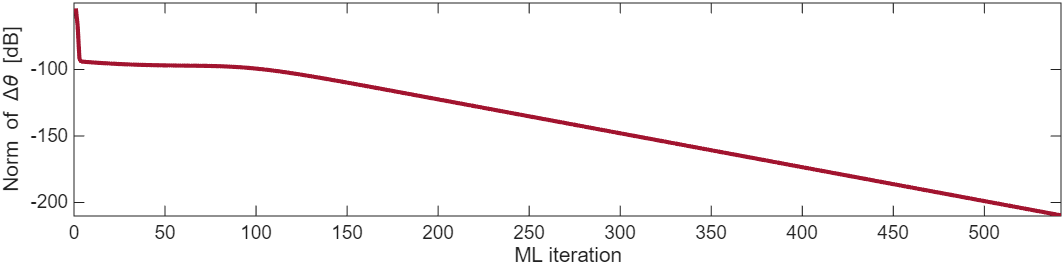
\includegraphics[width=0.48\textwidth]{Pictures/ML_theta_norm.png}
    \caption{Norm of the parameter change in function of the iteration for the optimal order of the ML algorithm.}
    \label{fig:delta_theta_norm}
\end{figure}









\section{Model Order Selection}
\label{sec:AIC}

The estimators described in Sec.~\ref{sec:parametric_model} require a model order $(n_a, n_b)$ to determine the right parameters $\theta = [a_0, \cdots, b_{n_b}]$ of~(\ref{eq:TF_general_form}).

The AIC criterion is therefore used. It depends on the cost of the estimator $V_{\text{est}}$ and the order of the model, giving an \textit{AIC cost}, given by
\begin{equation}
    V_{\text{AIC}} = V_{\text{est}} \Bigg( 1 + \frac{n_a + n_b}{N_e} \Bigg).
    \label{eq:AIC_cost}
\end{equation}
This is computed for various values of $n_a$ and $n_b$ and the optimal order is the one with the smallest \textit{AIC cost}.

The values of the order are restricted to transfer functions with more poles than zeros ($\Rightarrow n_a \geqslant n_b$) to have a stable system.

\section{Results}

The AIC criterion described in Sec.~\ref{sec:AIC} has been applied\footnote{for $n_a$ and $n_b$ going up to $15$.} to every estimator of Sec.~\ref{sec:parametric_model} and it gives for each of them a 3D plot like the one shown in Fig.~\ref{fig:AIC_3D}.

\begin{figure}
    \centering
    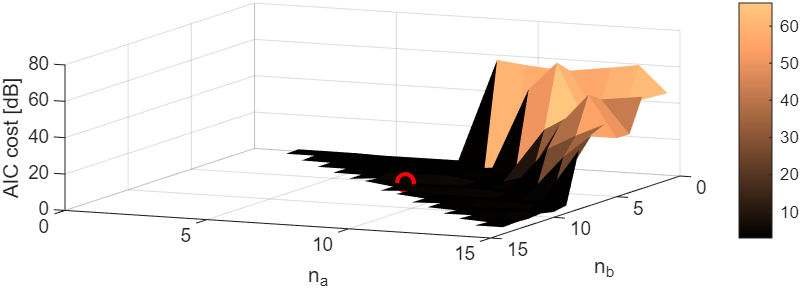
\includegraphics[width=0.48\textwidth]{Pictures/AIC_TLS.png}
    \caption{AIC cost depending on the order of the transfer function for the TLS estimator. The optimal order is circled in red.}
    \label{fig:AIC_3D}
\end{figure}

The resulting FRFs are plotted in Fig.~\ref{fig:estimated_FRF}. It can be seen that the LLS and TLS estimators have \textit{bumps} where poles and zeros nearly cancel each other's. The three last estimators (GTLS, BTLS and ML) superpose perfectly, making them undistinguishable on the graph.

\begin{figure}
    \centering
    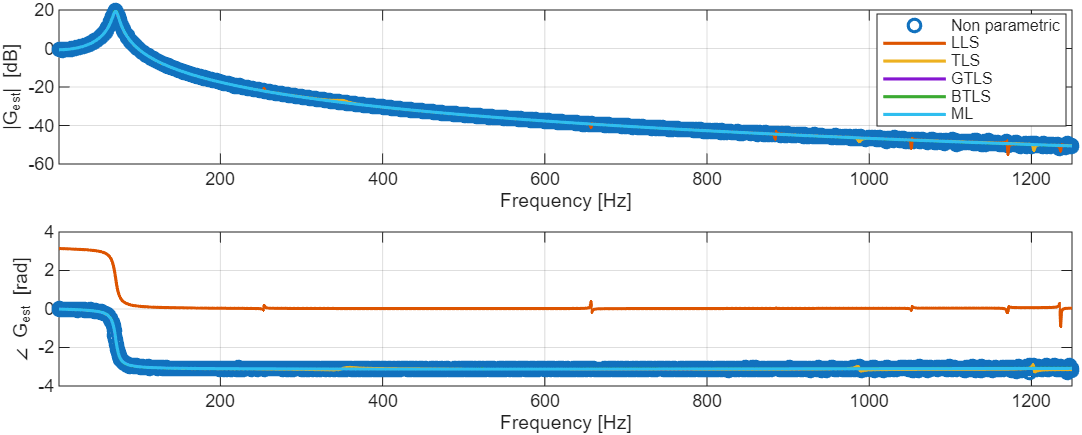
\includegraphics[width=0.48\textwidth]{Pictures/EstimatedFRF.png}
    \caption{Superposition of the estimated parametric FRFs amplitude (top) and phase (bottom), together with the nonparametric estimate.}
    \label{fig:estimated_FRF}
\end{figure}

Fig.~\ref{fig:optimal_order} shows the optimal order that minimizes the AIC cost~(\ref{eq:AIC_cost}). A few observations can be made:
\begin{itemize}
    \item The LLS and TLS estimators both have a high number of parameters and lay close to the limit $n_a = n_b$. Fig.~\ref{fig:rlocus1} confirms the hypothesis of imperfect pole-zero cancellations emitted based on the bumps of the FRF.
    \item GTLS and BTLS have a more intermediate number of parameters.
    \item The ML estimator uses a really low number of poles and zeros, yet achieve a performance similar to the GTLS on Fig.~\ref{fig:estimated_FRF}, which was expected as it is mathematically the best estimator.
\end{itemize}

\begin{figure}
    \centering
    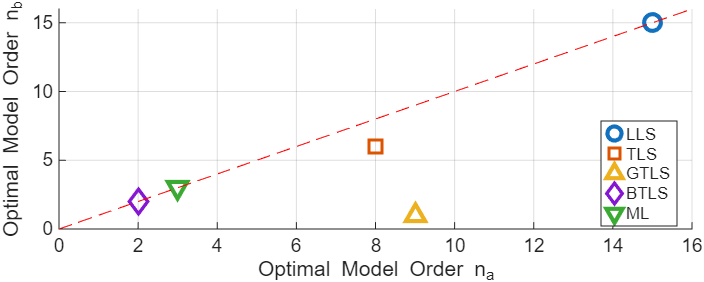
\includegraphics[width=0.48\textwidth]{Pictures/optimalOrder.png}
    \caption{Optimal orders for each estimator, according to the AIC criterion. The red dashed line is the stability limit $n_a = n_b$.}
    \label{fig:optimal_order}
\end{figure}

\begin{figure}
    \centering
    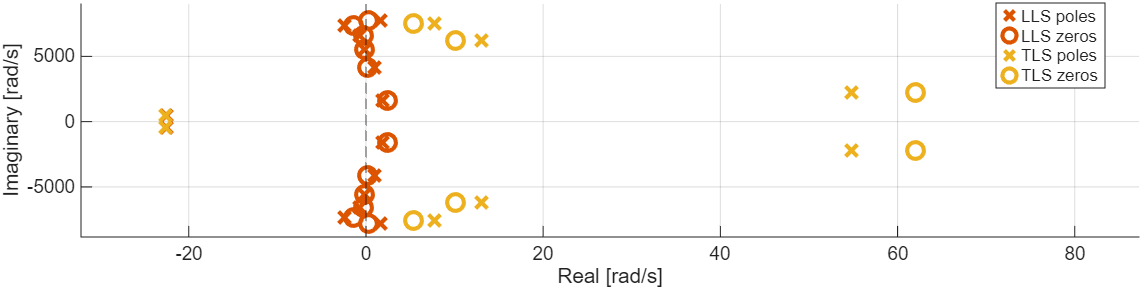
\includegraphics[width=0.48\textwidth]{Pictures/rlocus1.png}
    \caption{Poles and zeros of the LLS and TLS estimators. Only the ones close to the origin are shown to visualize the near pole-zero cancellation.}
    \label{fig:rlocus1}
\end{figure}

\begin{figure}
    \centering
    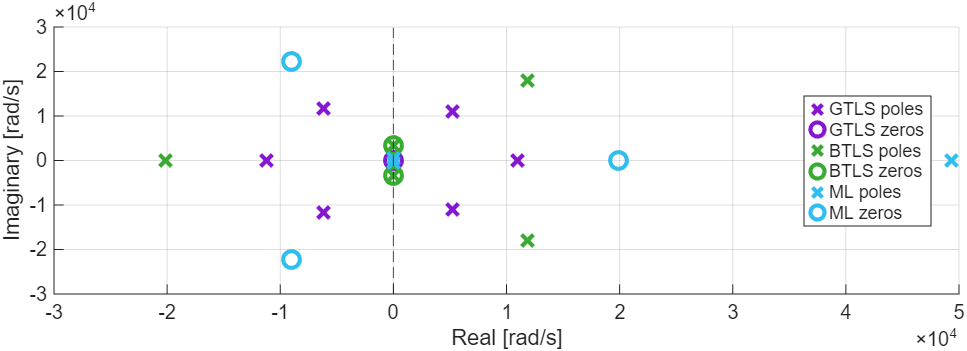
\includegraphics[width=0.48\textwidth]{Pictures/rlocus2.png}
    \caption{Poles and zeros of the GTLS, BTLS and ML estimators.}
    \label{fig:rlocus2}
\end{figure}

Finally, the poles and zeros of the GTLS, BTLS and ML estimators are shown in Fig.~\ref{fig:rlocus2}. It is here clearly visible that the GTLS estimator has poles in the right half-plane at high frequency, meaning the resulting system is unstable. Every estimator has poles with a positive real part but those of the ML and BTLS estimators are around $20$~rad/s, which is by far \textit{less unstable} than the one above $1000$~rad/s of the GTLS.

\section{Deeper Analysis of the Poles}

\subsection{Poles position uncertainty}

The covariance of the poles (and zeros) of the ML estimator can be approximated. First, the covariance of the parameters must be computed with
\begin{equation}
    \text{cov}(\theta_{\text{ML}}) \simeq 2 \Big(J_{\text{re}}^H J_{\text{re}}\Big)^{-1}.
\end{equation}

The covariance of the poles is then given by
\begin{equation}
    \text{cov}(p) = \frac{dp}{d\theta_{\text{ML}}} \text{cov}(\theta_{\text{ML}}) \frac{dp^H}{d\theta_{\text{ML}}},
\end{equation}
where $\frac{dp}{d\theta_{\text{ML}}}$ is based on how the parameters $[a_0, \cdots, a_{n_a}]$ relate to the poles $[p_0, \cdots, p_{n_a}]$.

The resulting standard deviation on the real part of the two poles in the right half-plane was really low as shown in Table~\ref{tab:pole_stddev}, meaning the estimator evaluates those close to their optimal positions. 

\begin{table}[h!]
    \centering
    \caption{Standard Deviation of Identified Poles, in rad/s}
    \begin{tabular}{|c|c|}
    \hline
    \textbf{Real Part} & \textbf{Imaginary Part} \\
    \hline
    $14.578 \times 10^3$ & $0$ \\
    $0.186$ & $0.185$ \\
    $0.186$ & $0.185$ \\
    \hline
    \end{tabular}
    \label{tab:pole_stddev}
\end{table}

For reference, the third pole of the ML estimator, which is visible on the extreme left of Fig.~\ref{fig:rlocus2} has a standard deviation of $\approx 14500$~rad/s. An expected result is the uncertainty on the imaginary port of this pole. Because it is alone, it lays on the real axis and the computed variance is exactly zero. These two clues combined implies that there is definitely a pole on the real axis, but it's exact frequency cannot be extracted from the measured data.

\subsection{Stable ML Estimator}
\label{sec:Stable_estimator}

To obtain a parametric FRF estimate with a stable model, the model~(\ref{eq:TF_general_form}) is replaced by:
\begin{equation}
    G(s) = \frac{\sum_{k=0}^{n_b} b_k s^k}{\prod_{k=1}^{n_a} (s-\alpha_k)}.
    \label{eq:TF_stable_model}
\end{equation}
With now $\theta = [\theta_\alpha \quad \theta_b]^T$, the poles are a direct parameter and they can be constrained. Before looking to the way of constraining them, let's see how the use of the new model~(\ref{eq:TF_stable_model}) impacts the ML algorithm briefly described in Sec.~\ref{sec:ML}.

$B_k$ and it's derivatives stay unchanged, except that the length of $\theta$ now becomes $n_a+n_b+1$, because explicitly writing the poles removes a parameter\footnote{It is worth noticing that this allows to remove the constraint on $||\theta||_2^2$, without which the the cost function was unconstrained because of the extra degree of freedom ($n_a+n_b+2$ parameters).}. On the other hand, we now have
\begin{equation}
    A_k = \prod_{i} (s_k-\alpha_i),
\end{equation}
and it's gradient along $\theta_\alpha$:
\begin{equation}
    \frac{\partial A_k}{\partial \theta_\alpha} = - A_k \begin{bmatrix}
        \frac{1}{(s_k - \alpha_1)} & \cdots & \frac{1}{(s_k - \alpha_{n_a})}
    \end{bmatrix}^T.
\end{equation}
Once the parameters update is computed by~(\ref{eq:ML_update}), $\Delta \theta$ is scaled such that the poles stay in the left half-plane. It is implemented as follows:
\begin{equation}
    \theta^{i+1} = \theta^i + k \Delta \theta
\end{equation}
where 
\begin{equation}
    k = \min\Bigg(1, \frac{-\Re\Big\{\alpha_j^ i\Big\}}{\Re\Big\{\alpha_j^{i+1}\Big\} - \Re\Big\{\alpha_j^i\Big\}}\Bigg)
    \label{eq:delta_theta_limit}
\end{equation}
for every pole $\alpha_j$ such that $\Re\Big\{\alpha_j^{i+1}\Big\} > 0$. A second approach could have been to limit only the poles that would cross the imaginary axis but this would have been equivalent to not follow the gradient anymore, losing the interest of using a maximum likelihood estimator. The resulting FRF is compared with the one obtained without constraining the poles in Fig.~\ref{fig:FRF_stable_ML}.

\begin{figure}
    \centering
    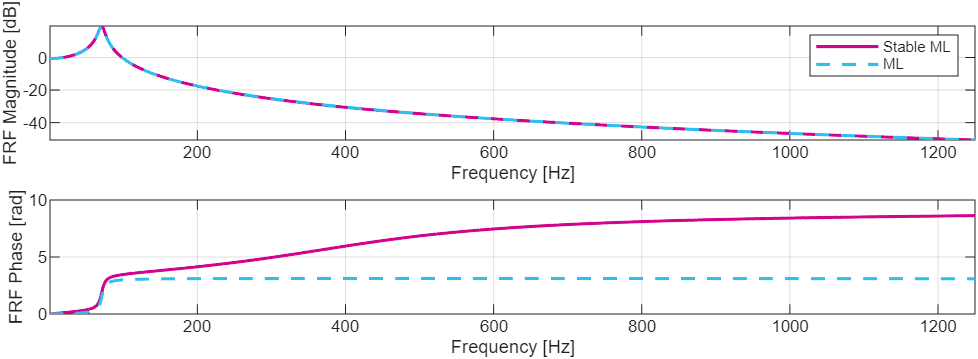
\includegraphics[width=0.48\textwidth]{Pictures/FRF_stable_ML.png}
    \caption{Comparison of the estimated FRF of the ML and the stable ML algorithms.}
    \label{fig:FRF_stable_ML}
\end{figure}

This estimator, called \textit{stable ML} is however not useful. If it does impose poles with a negative real value, it cannot be applied while enforcing real parameters as the poles $\alpha_1, \cdots, \alpha_{n_a}$ need to be complex. The resulting parameter vector can therefore not be written again in the general form~(\ref{eq:TF_general_form}) with real values for $a_k$ and $b_k$.

\subsection{Stable Real ML Estimator}
\label{sec:stable_real_estimator}

This section starts from what has been done is Sec.~\ref{sec:Stable_estimator} and improves it to end up with real parameters, while maintaining stable poles, hence the name \textit{Stable Real ML} estimator.

The transfer function takes the form
\begin{equation}
    G(s) = \frac{\sum_{k=0}^{n_b} b_k s^k}{\prod_{k=1}^{n_{a, \text{re}}} (s-a_k) \prod_{k=1}^{n_{a, \text{cplx}}} (s^2 - 2 s \alpha_k \cos \phi_k + \alpha_k^2)},
    \label{eq:TF_stable_real_model}
\end{equation}
such that it's poles are given by $a_k$ and $\alpha_k e^{\pm j \phi_k}$. The parameters have now become 
\begin{equation}
    \theta = \begin{bmatrix}
        a_k & \alpha_k & \phi_k & b_k
    \end{bmatrix}^T.
    \label{eq:theta_stable_real}
\end{equation}
This new model implies the following changes:
\begin{gather}
    A_k = \prod_{i} (s_k-a_i) \prod_{i} (s_k^2 - 2 s_k \alpha_i \cos \phi_i + \alpha_i^2),\\
    \frac{\partial A_k}{\partial \theta_a} = -A_k \begin{bmatrix}
        \cdots & \frac{1}{(s_k-a_i)} & \cdots
    \end{bmatrix}^T,\\
    \frac{\partial A_k}{\partial \theta_\alpha} = 2 A_k \begin{bmatrix}
        \cdots & \frac{\alpha_i - s_k \cos \phi_i}{(s_k^2 - 2 s_k \alpha_i \cos \phi_i + \alpha_i^2)} & \cdots
    \end{bmatrix}^T, \\
    \frac{\partial A_k}{\partial \theta_\phi} = 2 A_k \begin{bmatrix}
        \cdots & \frac{s_k \alpha_i \sin \phi_i}{(s_k^2 - 2 s_k \alpha_i \cos \phi_i + \alpha_i^2)} & \cdots
    \end{bmatrix}^T.
\end{gather}
This model allows complex poles which are complex conjugates, while keeping the parameters real. However, constraining the poles to the left half-plane is still done by limiting $\Delta \theta$ with~(\ref{eq:delta_theta_limit}), which truncates the set of acceptable solutions in an artificial way.

Before adding another layer of complexity to cure this, let's rapidly discuss the results of this estimator. The optimal order is way higher than the one computed by the ML estimator. However, there is no big difference between the optimal AIC cost and the one on the flat region at lower orders, as shown on Fig.~\ref{fig:AIC_stable_real_ML}. The hope is that an improved model might be able to reach a lower cost in the region of lower order.

The final ML cost of all the maximum likelihood estimators, computed with~(\ref{eq:ML_cost}), are shown in Table~\ref{tab:ML_costs}. The stable real ML estimate shown on Fig.~\ref{fig:FRF_stable_real_ML} is already a better match than Fig.~\ref{fig:FRF_stable_ML}, which is surprising as the set of admissible solutions is reduced by imposing complex conjugate poles and zeros. 

\begin{table}
    \centering
    \caption{Maximum Likelihood Cost Comparison}
    \begin{tabular}{|c|c|}
    \hline
    \textbf{Estimator} & \textbf{ML Cost} \\
    \hline
    ML & $822$ \\
    Optimal ML & $25\,345$ \\
    Stable Real ML & $27\,107$ \\
    Stable ML & $35\,941$ \\
    \hline
    \end{tabular}
    \label{tab:ML_costs}
\end{table}

To explain why it performs better than the stable ML estimator, it could be that the jacobian pushes the poles to the right half-plane, which violates the constraints faster for the latter and stops it at a higher cost.

\begin{figure}
    \centering
    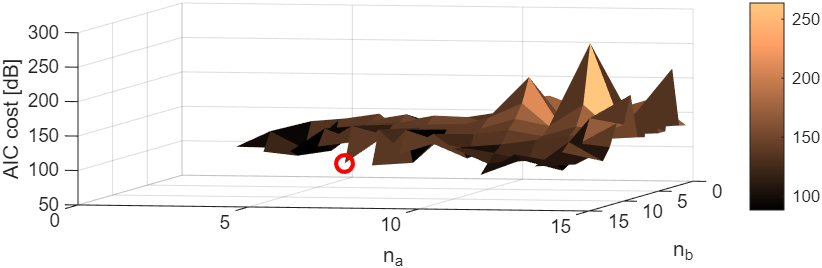
\includegraphics[width=0.48\textwidth]{Pictures/AIC_stable_real_ML.png}
    \caption{AIC cost of the stable real ML estimator. The optimal order is circled in red.}
    \label{fig:AIC_stable_real_ML}
\end{figure}

\begin{figure}
    \centering
    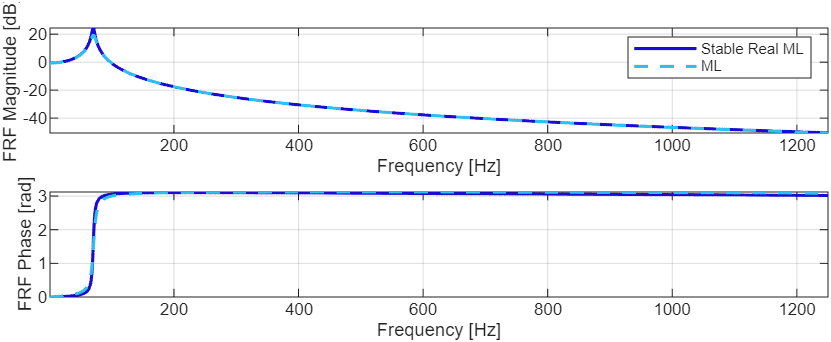
\includegraphics[width=0.48\textwidth]{Pictures/FRF_stable_real_ML.png}
    \caption{Comparison of the estimated FRF of the ML and the stable real ML algorithms.}
    \label{fig:FRF_stable_real_ML}
\end{figure}

\subsection{Optimal ML Estimator}

This estimator is called \textit{optimal ML} as it removes the need for hand crafted constraints. This is done by manipulating~(\ref{eq:TF_stable_real_model}) so its poles can no longer have a positive real part. It results in
\begin{equation}
    G(s) = \frac{\sum_{k=0}^{n_b} b_k s^k}{\prod_{k=1}^{n_{a, \text{re}}} (s+a_k^2) \prod_{k=1}^{n_{a, \text{cplx}}} (s^2 + 2 s \alpha_k^2 + \alpha_k^4 + \phi_k^2)},
    \label{eq:TF_optimal_model}
\end{equation}
and for the same parameter vector $\theta$ as in~(\ref{eq:theta_stable_real}),
\begin{gather}
    A_k = \prod_{i} (s_k+a_i^2) \prod_{i} (s_k^2 + 2 s_k \alpha_i^2 + \alpha_i^4 + \phi_i^2),\\
    \frac{\partial A_k}{\partial \theta_a} = 2 A_k \begin{bmatrix}
        \cdots & \frac{a_i}{(s_k+a_i^2)} & \cdots
    \end{bmatrix}^T,\\
    \frac{\partial A_k}{\partial \theta_\alpha} = 2 A_k \begin{bmatrix}
        \cdots & \frac{s_k\alpha_i + 2\alpha_i^3}{(s_k^2 + 2 s_k \alpha_i^2 + \alpha_i^4 + \phi_i^2)} & \cdots
    \end{bmatrix}^T, \\
    \frac{\partial A_k}{\partial \theta_\phi} = 2 A_k \begin{bmatrix}
        \cdots & \frac{\phi_i}{(s_k^2 + 2 s_k \alpha_i^2 + \alpha_i^4 + \phi_i^2)} & \cdots
    \end{bmatrix}^T.
\end{gather}

To conclude the presentation of this estimator, it uses as initial parameters the results of the stable real ML estimator of Sec.~\ref{sec:stable_real_estimator}.

Even though it was never mentioned in this report, the norm of $\Delta \theta$ at the end of the Newton-Gauss iteration has always been checked and was determined to be low enough so a second loop using the Levenberg-Marquardt (LM) algorithm was never used.

This norm was however not negligible with this optimal ML estimator so the LM was implemented and "retro-fitted" to every ML estimator. The most complicated part was the determination of a convergence condition and it was decided to be a minimal threshold on the relative change of the parameters:
\begin{equation}
    \frac{||\Delta\theta||}{||\theta||} \leq 10^{-12}
\end{equation}

The cost improve between the stable real estimator and this one is quite small, as shown in Table~\ref{tab:ML_costs}. Visually, the phase estimate is way worse going from Fig.~\ref{fig:FRF_stable_real_ML} to Fig.~\ref{fig:FRF_optimal_ML} but the overshoot at the oscillation frequency is lower, resulting in a smaller cost.

\begin{figure}
    \centering
    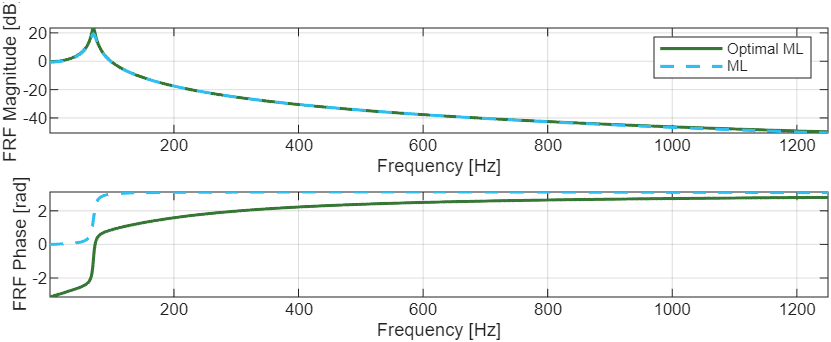
\includegraphics[width=0.48\textwidth]{Pictures/FRF_optimal_ML.png}
    \caption{Comparison of the estimated FRF of the ML and the optimal ML algorithms.}
    \label{fig:FRF_optimal_ML}
\end{figure}

The optimal orders of the ML estimators shown on Fig.~\ref{fig:optimal_order_ML} show that the stable real ML estimate is still a decent choice of model as its ML cost is close to the one of the optimal ML but it needs 2 parameters less.

\begin{figure}
    \centering
    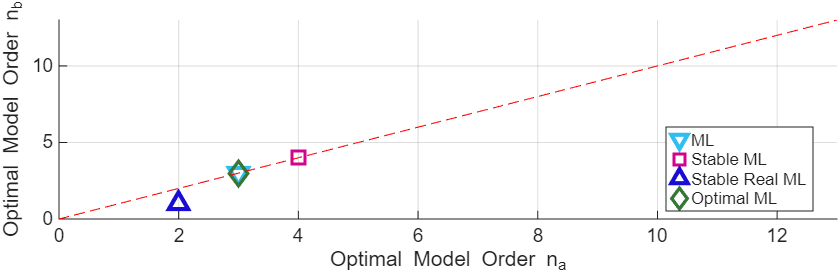
\includegraphics[width=0.48\textwidth]{Pictures/optimalOrderML.png}
    \caption{Optimal orders for each variant of the ML estimator, according to the AIC criterion. The red dashed line is the stability limit $n_a = n_b$.}
    \label{fig:optimal_order_ML}
\end{figure}

A final note can be made about the uncertainty on the poles of the SRML and OML estimators. Their expressions link directly the parameters to the poles so their gradients $\partial p / \partial \theta$ are block matrices. They are structurally described here, just to give an insight on how they are built.
\begin{gather}
    \frac{\partial p_{\text{SRML}}}{\partial \begin{bmatrix}
        \theta_a & \theta_\alpha & \theta_\phi
    \end{bmatrix}} = \begin{bmatrix}
        I & &\\
        & \text{diag}_i \Big(e^{j\phi_i}\Big) & \text{diag}_i \Big(j\alpha_i e^{j\phi_i}\Big)\\
        & \text{diag}_i \Big(e^{-j\phi_i}\Big) & \text{diag}_i \Big(-j\alpha_i e^{-j\phi_i}\Big)\\
    \end{bmatrix} \notag \\
    \frac{\partial p_{\text{OML}}}{\partial \begin{bmatrix}
        \theta_a & \theta_\alpha & \theta_\phi
    \end{bmatrix}} = \begin{bmatrix}
        \text{diag}_i \Big(-2a_i\Big) & &\\
        & \text{diag}_i \Big(-2\alpha_i\Big) & j I\\
        & \text{diag}_i \Big(-2\alpha_i\Big) & -j I\\
    \end{bmatrix} \notag 
\end{gather}

And finally, the resulting standard deviation of the poles are given in Table~\ref{tab:ML_pole_stddev}. It can be observed that the standard deviation of the complex conjugate poles (responsible for the oscillation) of the OML estimator is higher than with SRML. 

\begin{table}[h!]
    \centering
    \caption{Standard deviation of estimated poles for SRML and OML}
    \label{tab:ML_pole_stddev}
    \begin{tabular}{l c c}
    \hline
    \textbf{Estimator} & \textbf{Pole location} & \textbf{Std. deviation} \\
    \hline
    SRML 
    & $-12.1855 + j\,442.5608$ 
    & $0.1416 + j\,0.1165$ \\

    SRML 
    & $-12.1855 - j\,442.5608$ 
    & $0.1416 + j\,0.1165$ \\
    \hline
    OML 
    & $-1153.1149$ 
    & $22.7454$ \\

    OML 
    & $-14.1987 + j\,444.4559$ 
    & $0.3500 + j\,0.1980$ \\

    OML 
    & $-14.1987 - j\,444.4559$ 
    & $0.3500 + j\,0.1980$ \\
    \hline
    \end{tabular}
\end{table}

